\documentclass{standalone}
% translate with >> pdflatex -shell-escape <file>

% This file is an extract of the PGFPLOTS manual, copyright by Christian Feuersaenger.
% 
% Feel free to use it as long as you cite the pgfplots manual properly.
%
% See
%   http://pgfplots.sourceforge.net/pgfplots.pdf
% for the complete manual.
%
% Any required input files (for <plot table> or <plot file> or the table package) can be downloaded
% at
% http://www.ctan.org/tex-archive/graphics/pgf/contrib/pgfplots/doc/latex/
% and
% http://www.ctan.org/tex-archive/graphics/pgf/contrib/pgfplots/doc/latex/plotdata/

\usepackage{pgfplots}
\usepackage{pgfplotstable}
\pgfplotsset{compat=newest}

% The manual loads these libraries globally; the extracted standalone examples
% need them too. external/clickable/snakes are intentionally omitted.
\usetikzlibrary{
	arrows.meta,backgrounds,calc,decorations.footprints,decorations.markings,
	decorations.pathreplacing,fixedpointarithmetic,intersections,patterns,
	plotmarks,shapes.arrows,spy,through}
\usepgfplotslibrary{
	colorbrewer,colormaps,dateplot,fillbetween,groupplots,patchplots,polar,
	smithchart,statistics,ternary,units}

% Some colormap examples reuse this display style defined earlier in the manual.
\pgfplotsset{
	cycle from colormap manual style/.style={
		x=3cm,y=10pt,ytick=\empty,
		colorbar style={x=,y=,ytick=\empty},
		point meta min=0,point meta max=1,
		stack plots=y,
		y dir=reverse,colorbar style={y dir=reverse},
		every axis plot/.style={line width=2pt},
		legend entries={0,...,20},
		legend pos=outer north east,
	},
}

\pagestyle{empty}

\usepgfplotslibrary{groupplots}
\usepgfplotslibrary{groupplots}

\begin{document}
% Example using groupplots library
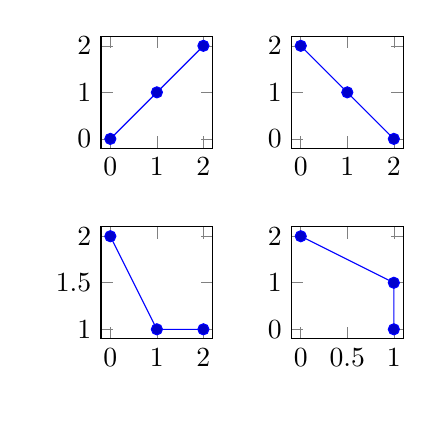
\begin{tikzpicture}
    \begin{groupplot}[group style={group size=2 by 2},height=3cm,width=3cm]
    \nextgroupplot
        \addplot coordinates {(0,0) (1,1) (2,2)};
    \nextgroupplot
        \addplot coordinates {(0,2) (1,1) (2,0)};
    \nextgroupplot
        \addplot coordinates {(0,2) (1,1) (2,1)};
    \nextgroupplot
        \addplot coordinates {(0,2) (1,1) (1,0)};
    \end{groupplot}
\end{tikzpicture}
    \qquad
% Same example created as done without the library
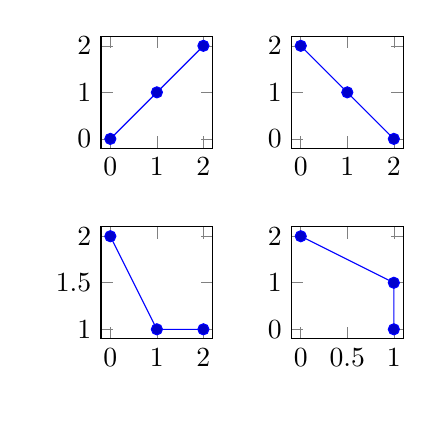
\begin{tikzpicture}
    \begin{axis}[name=plot1,height=3cm,width=3cm]
        \addplot coordinates {(0,0) (1,1) (2,2)};
    \end{axis}
    \begin{axis}[name=plot2,at={($(plot1.east)+(1cm,0)$)},anchor=west,height=3cm,width=3cm]
        \addplot coordinates {(0,2) (1,1) (2,0)};
    \end{axis}
    \begin{axis}[name=plot3,at={($(plot1.south)-(0,1cm)$)},anchor=north,height=3cm,width=3cm]
        \addplot coordinates {(0,2) (1,1) (2,1)};
    \end{axis}
    \begin{axis}[name=plot4,at={($(plot2.south)-(0,1cm)$)},anchor=north,height=3cm,width=3cm]
        \addplot coordinates {(0,2) (1,1) (1,0)};
    \end{axis}
    \end{tikzpicture}
\end{document}
